\documentclass[11pt,a4paper,portrait]{article}
\usepackage[utf8]{inputenc}
\usepackage{amsmath}
\usepackage{amsfonts}
\usepackage{amssymb}
\usepackage{titling}
\usepackage[
backend=bibtex,
style=science,
sorting=none
]{biblatex}
\usepackage[utf8]{inputenc}
\usepackage[english]{babel}
\usepackage{graphicx}

\title{Information Processing with DNA}
\author{Candidate Number: 6892V. Supervisor: Dr. Ulrich F. Keyser}
\addbibresource{bibliography}
\begin{document}
\begin{titlingpage}
\maketitle
	
\begin{abstract}
Information processing using DNA is a recent development in the field of biology/computing and has many exciting applications. Three techniques are looked at in detail in this report, each technique has been used to process information using DNA by creating Boolean logic gate like devices. The first of which is Deoxyribozyme based, computations are carried out by introducing oligonucleotides which act as allosteric effectors for the Deoxyribozyme logic gate producing a conformational change (shape change) they can act as inhibitors or activators. The output is the presence or absence of an output oligonucleotide that is produced when the Deoxyribozyme cleaves a substrate \cite{DeoxyribozymeLogic}. Another method that is discussed is enzyme free, this method uses the principle of strand displacement to carry out computation. Input oligonucleotides bind at toehold regions on the logic gate and can displace other strands to expose further toeholds or they can release an output oligonucleotide \cite{enzymefree}. The last method that is discussed is a tiling method in which outputs and inputs are encoded as a specific DNA motif (DNA triple crossover tiles in this case) that can only bind to other specific tiles. Using this method cumulative logical operations can be carried out (XOR) \cite{Tiles00}. Applications of these methods include general computation in vivo \cite{Qian11}, smart therapeutics (targeted drug delivery) \cite{Aptamer}, and the algorithmic generation of patterns/smart-materials\cite{Tiles00} \cite{Sierpinski}. Several implementations that demonstrate these applications are discussed.
\end{abstract}
	
\end{titlingpage}

\clearpage
\section{Introduction}

Richard Feynman first proposed "Subatomic computers" in 1959, so could be credited with kick-starting the idea of molecular computing \cite{Feynmann}. But the birth of the field (DNA computing) is often regarded as stemming from Leonard Adleman's original paper published in 1994 \cite{Adleman1994}. However there have been significant developments in the field since this paper was released. DNA computing is a wonderful technique that may find uses in a variety of applications in the future including long term storage solutions \cite{Cox2001}, smart therapeutics (in vivo) \cite{Qian11}, and solving general computing tasks that may benefit from the massive parallelisation provided \cite{Adleman1994}\cite{Ezziane06}.
\\ \\

This report will mention the advantages and disadvantages of information processing with DNA and will discuss and evaluate several of the techniques that have been used to create Boolean logic gate like devices. It shall also describe various interesting implementations of such techniques and some of their possible applications. It is hoped that this report will be accessible to the general reader so a brief section defining important terms and explaining useful techniques is provided.

\newpage
\subsection{Adleman's Original Paper}
In this paper Adleman demonstrated a solution to the directed Hamiltonian problem. Which is a problem in Graph theory that aims to find a solution to the problem of finding a route connecting a starting vertex to an ending vertex that travels through all of the other vertices in the graph. The directed problem has certain vertices connected by directional paths \cite{Hamiltonian}. In the paper Adleman describes a method he developed to solve this problem using "standard protocols", DNA, and enzymes \cite{Adleman1994}.

\begin{figure}[ht!]

\centering
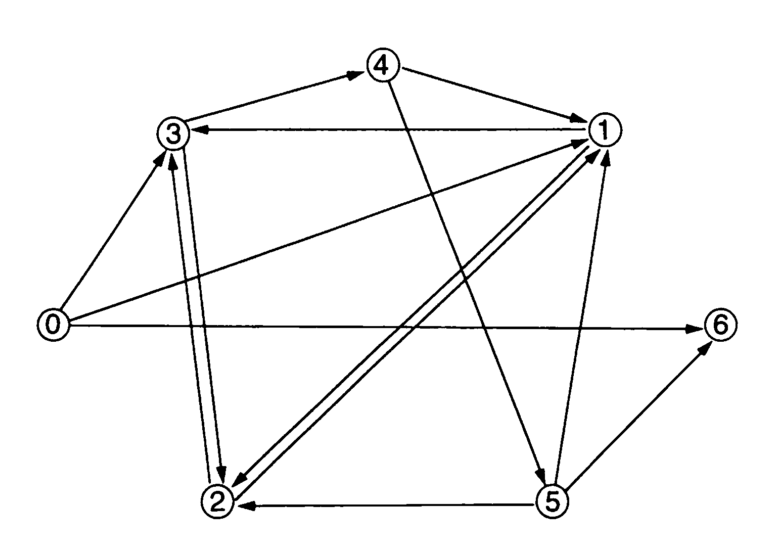
\includegraphics[width=60mm, height=60mm]{hamiltonianpath.png}
\caption{Example of a directed Hamiltonian problem. Routes are directed and connect a starting vertex to an allowed ending vertex. Route starts at vertex 0 and ends at vertex 6. Solution is $0 \rightarrow 1 \rightarrow 2 \rightarrow 3 \rightarrow 4 \rightarrow 5 \rightarrow 6$. \cite{Adleman1994}
\label{hamiltoniangraph}}
\end{figure}

The aim of Adleman was to solve the graph described in Figure ~\ref{hamiltoniangraph}. To do this Adleman synthesised 7 unique 20 base long DNA strands that were each associated with a single vertex in the graph. The paths between a vertex i to a vertex j ($i \rightarrow j$) is represented by a 20 base length DNA strand with the first 10 bases the same as the last 10 bases of vertex i, and the last 10 bases the same as the first 10 bases of vertex j. There are a few special vertex-vertex path cases but the general idea is the same. Adleman mixed strands complementary to the vertex oligonucleotides with strands corresponding to the paths between vertices. Due to how the particular strands were constructed, and the tendency for DNA to form double helices between complementary strands random paths through the graph are constructed. The complementary vertex strands act as connections between compatible paths connecting path strands to form a complete Hamiltonian path through the graph. This can obviously be scaled up to include problems with many more vertices and paths by creating the corresponding oligonucleotides. Although Adleman does admit in his paper that this method may not apply the most efficient algorithm \cite{Adleman1994}.
\\\\
After the strands mix and create the random paths through the graph he carried out PCR using primers corresponding to the 0 vertex and complementary to the 6 vertex. The selection of these primers means that only paths starting at the 0 vertex and ending at the 6 vertex are amplified. This vastly reduces the remaining paths in the solution space. The amplified strands are then run through gel electrophoresis to select only double strands which are 140bp long, this is so that only paths containing 7 vertices are kept as possible solutions. The remaining solutions are then PCR amplified. The solutions are then affinity purified by incubating the strands with bound complementary vertex strands successively to select only the solutions containing all 7 vertices \cite{Adleman1994}.
\\\\

The remaining strands are thus the solutions to the directed Hamiltonian path problem described in Figure ~\ref{hamiltoniangraph}, using standard sequencing techniques you can determine these solutions \cite{Adleman1994}.
\\\\

\clearpage
\section{Basics}
\subsection{DNA}
DNA (Deoxyribonucleic acid) is a molecule that encodes genetic information, DNA is usually found as a double strand (Double-Helix). However single strands can exist independently. A single DNA strand contains multiple nucleotides which are constructed from a negatively charged phosphate group (making DNA negatively charged), a sugar (deoxyribose) and a nitrogenous base (\textbf{A}denine, \textbf{T}hymine, \textbf{C}ytosine, \textbf{G}uanine). Deoxyribose contains 5 carbon atoms which are labelled 1'$\rightarrow$5'. The phosphate group is attached to the 5' Carbon and the base is attached to the 1' Carbon. The 3' Carbon has a hydroxyl group (OH) attached to it. 

\begin{figure}[ht!]
\centering
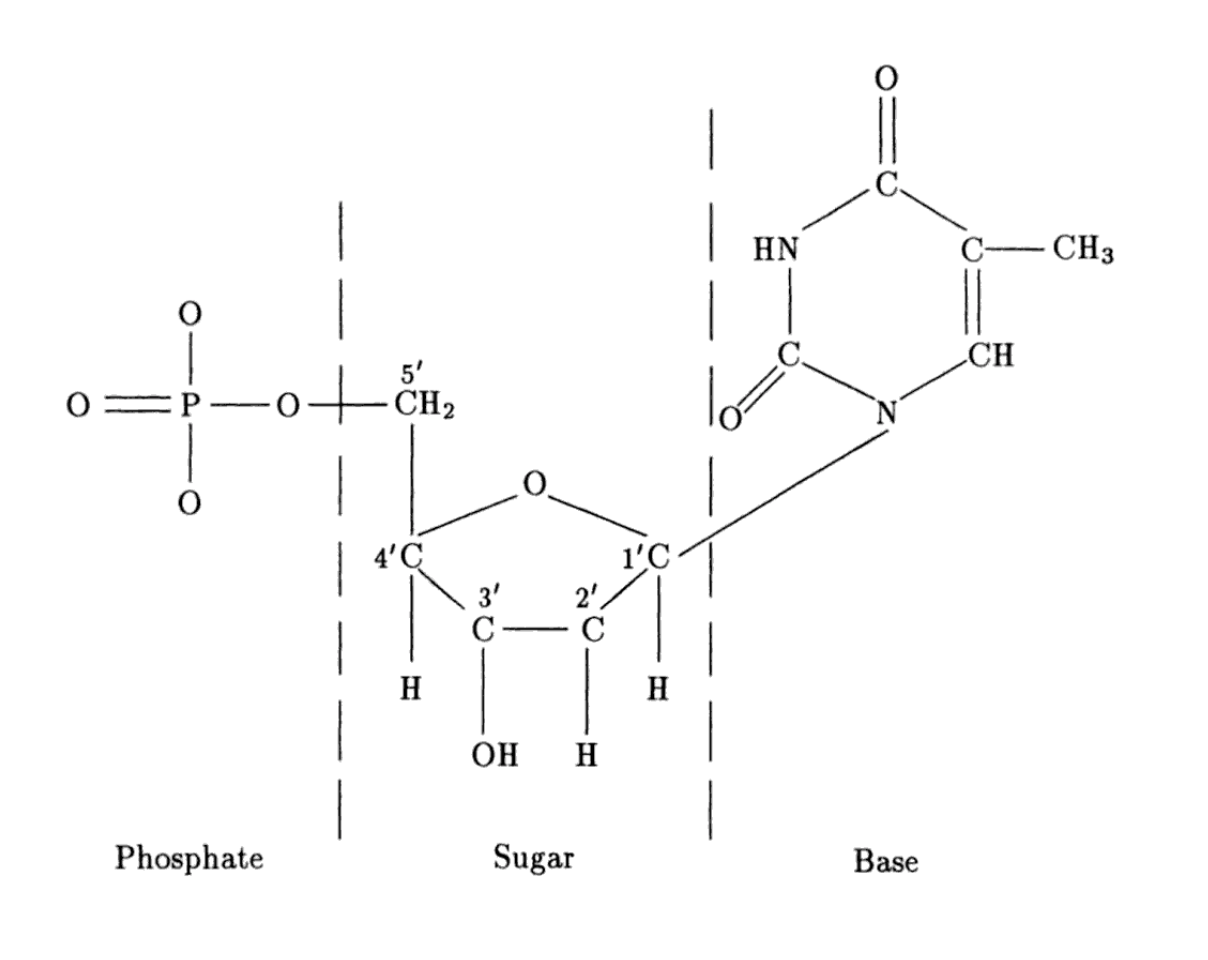
\includegraphics[width=60mm, height=60mm]{nucleotide.png}
\caption{Chemical structure of a nucleotide (Thymine base) \cite{paun2013DNA}. \label{nucleotide}}
\end{figure}

Double strands are held together by Hydrogen bonds, which can only form between complementary base pairs (2 between \textbf{A\&T} and 3 between \textbf{C\&G}). Phosphodiester bonds (strong covalent bonds) bind the nucleotides in individual strands together, they join the phosphate group at 5' on one nucleotide with the 3'-OH group on another nucleotide. In a DNA strand there is therefore one side with the 3'-OH group available and another with the 5'-phosphate group available, giving DNA a directionality \cite{paun2013DNA}. 

Because hydrogen bonds are much weaker than phosphodiester bonds it is possible to separate double strands without breaking the individual structure of each strand by raising the temperature.
\clearpage
\begin{figure}[ht!]
\centering
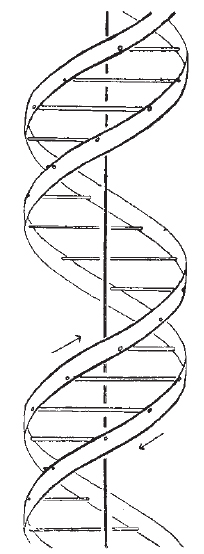
\includegraphics[width=40mm, height=50mm]{helix.jpg}
\caption{Illustration of DNA's helical structure \cite{watsoncrick} \label{dnafig}}
\end{figure}

A single strand of DNA is capable of folding in to secondary and tertiary structures. Some of these structures allow the binding of substrates and may be able to function as catalysts (enzymes) \cite{dnaenzyme}.

\subsection{DNA Manipulation Techniques}
\textbf{Polymerase chain reaction (PCR)} -  is a technique used to create large quantities of DNA by replicating a specific template double strand. The double strand is broken apart and DNA polymerase attaches free nucleotides (triphosphate) to each single strand starting at the site of an annealed primer (oligonucleotides that bind to each single strand) to create multiple double stranded copies \cite{PCR}.
\\\\
\textbf{Gel Electrophoresis} - is a method used to sort DNA molecules by size by running them through a viscous gel using an electric field. The molecules are labelled using dyes or radioactive/fluorescent markers so that their locations in the gel can be determined \cite{dna}.

\subsubsection{Polymerase Chain Reaction - PCR}
PCR can be used to replicate specific strands of DNA (number of strands doubled after every cycle). PCR requires:
\begin{itemize}
   \item Template double strands - DNA sequence to be copied.
   \item Primers - oligonucleotides that hybridise to a sequence of complementary base pairs on each of the template strands.
   \item DNA Polymerase - enzyme that synthesizes a new strand by joining free nucleotides to the template starting from the binding location of the primer. Extends in the 5'-3' direction \cite{paun2013DNA}.
   \item Free Nucleotides (triphosphate) - composed of deoxyribose, three phosphate groups, and a nitrogenous base (\textbf{A, T, C or G}).
   \item Buffer - solution providing optimum conditions for the polymerase enyzmes. 
\end{itemize}

Instructions for a single cycle:
\begin{enumerate}
\item Heat the solution to a high enough temperature such that the Hydrogen-bonds between bases in the template strand break. Creating two single strands.
\item Lower the temperature to a level at which the primers can anneal to complementary bases on each of the single strands.
\item Finally set the temperature to the optimal value for the specific DNA polymerase that is used. This step joins the free nucleotides to the single strands, making each of them double stranded.
\end{enumerate}

These steps can be carried out multiple times to synthesise large quantities of DNA \cite{PCR}.

\subsubsection{Gel Electrophoresis}
Because DNA molecules are negatively charged they can be directed using an electric field. Placing DNA molecules in a viscous gel and applying an electric field across the gel causes the molecules to move towards the positive end of the gel. Because the gel is viscous larger DNA molecules will move more slowly than smaller ones, in this way DNA can be sorted by size (number of base pairs). Often DNA fragments of known size are sent through the gel to lay down markers. The fragments are labelled using dyes or radioactive/fluorescent markers so that they can be detected \cite{dna}.

\subsection{Fluorescence Resonance Energy Transfer - FRET}
A fluorescing method based on FRET is widely used by several DNA computing techniques for detection. In FRET a fluorescent donor is excited by a specific wavelength, this excitation energy is then absorbed by a fluorescent acceptor by a long-range dipole-dipole coupling mechanism. The donor then returns to the ground state. The efficiency of this energy transfer falls as $1/r^6$, so it is possible to detect when these molecules become separated as the emission spectrum from the donor becomes much more pronounced at larger separations \cite{Compbio}.

\clearpage
\section{Techniques and Developments}
\subsection{Deoxyribozymes}
It is possible to create logic gates based on Deoxyribozymes that can be chained together to compute any Boolean function using oligonucleotides as both inputs and outputs \cite{DeoxyribozymeLogic}. It is envisaged that these logic gates will be used to analyse disease markers in vivo and compute a response (release a drug etc.) \cite{LigaseLogic}.
\\\\
The output oligonucleotides contain a single ribonucleotide (rAdenosine) embedded in a deoxyribonucleotide chain. The difference between the two nucleotides is the sugar they contain, a ribonucleotide contains a ribose rather than a deoxyribose sugar. A ribose sugar contains an additional hydroxyl group on its 2' Carbon \cite{paun2013DNA}. The deoxyribozymes cleave the phosphodiester backbone of these oligonucleotides at the location of the ribonucleotide. The answer to a computation is the presence (true) or absence (false) of this cleaved oligonucleotide \cite{DeoxyribozymeLogic}. To detect the presence of the cleaved oligonucleotide a method based on FRET is used \cite{FRET}. The output oligonucleotide is labelled with a fluorescein donor at the 5' end, and with a tetramethylrhodamine acceptor at the 3' end. When the oligonucleotide has been cleaved a peak at 520nm is observed \cite{DeoxyribozymeLogic}. To create the logic gates stem loops (loops of single stranded DNA) are attached to the deoxyribozymes at their binding arms, these stem loops inhibit the function of the deoxyribozyme by blocking the recognition region, preventing substrate binding. When the input oligonucleotides are present they open the stem loops by bonding to the complementary bases inside the stem loop. Once open the recognition site becomes unblocked and the substrate can bond. Through careful design of stem loops various logic gates can be constructed \cite{DeoxyribozymeLogic}. If the structure of the deoxyribozyme allows it an additional stem loop may be placed within the catalytic core. When this stem loop is open (input oligonucleotide is present) the catalytic core is distorted and cleavage of the output molecule is inhibited. When the stem loop is closed cleavage remains uninhibited \cite{Stojanovic2014}. These inhibitory stem loops can be used to create a NOT gate (output molecule only cleaved when input molecule not present). 

\begin{figure}[bp!]
\centering
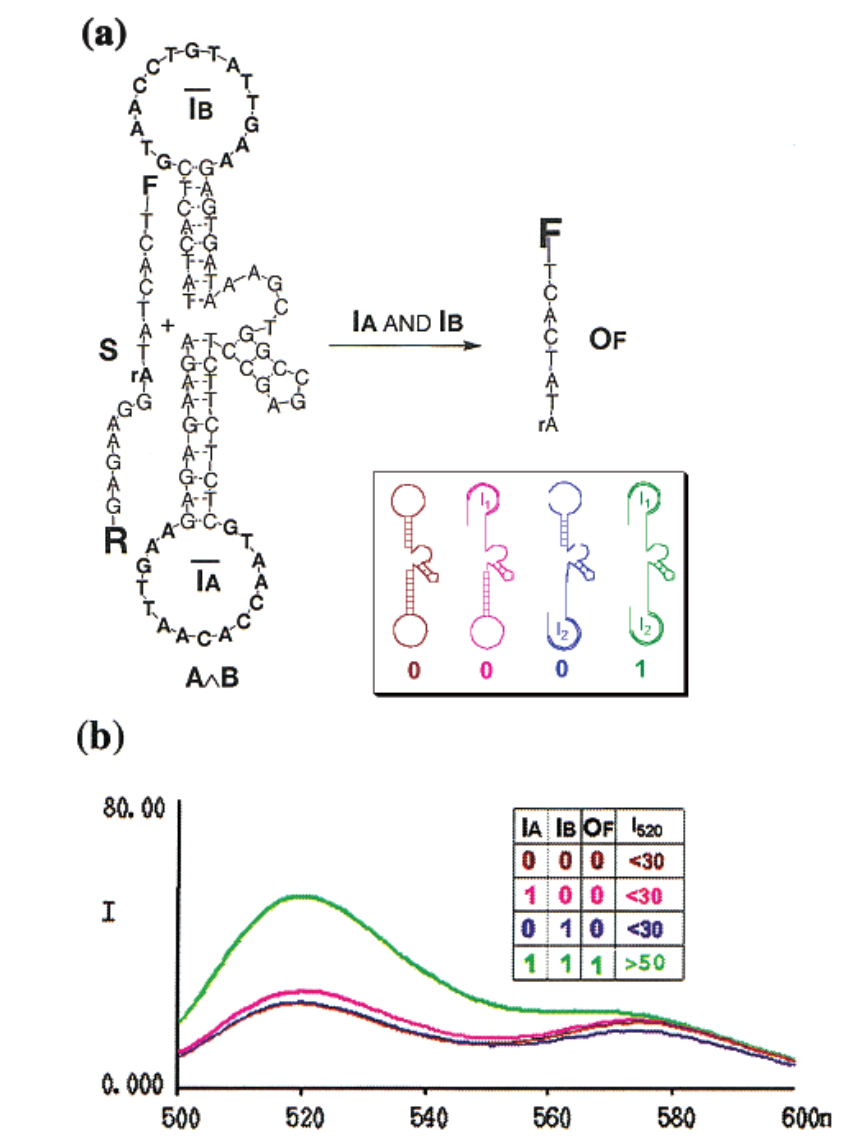
\includegraphics[width=80mm, height=80mm]{andgate.png}
\caption{ (a) Shows an AND gate with two stem loops complementary to input oligonucleotides $I_A$ and $I_B$, in its current configuration the binding site for the substrate S is blocked. In the presence of both $I_A$ and $I_B$ the stem loops open and S can bind. The deoxyribozyme can then cleave S at rA producing the output oligonucleotide $O_F$.(b) Shows the result of measurement, there is a peak at 520nm when both $I_A$ and $I_B$ are present. This is expected as when S has been cleaved the two oligonucleotides produced should separate, causing output at 520nm to be uninhibited. \cite{DeoxyribozymeLogic}}
\label{andgate}
\end{figure}
\clearpage
There have been several implementations that employ this technique for computation. A half-adder has been implemented. A half adder computes the sum of 2 input bits and returns a sum and a carry bit (for sum overflow 01b+01b=10b). Full adders can also be constructed. Full adders compute the sum of 3 bits and are an important component for constructing an arithmetic logic unit. A half adder can be constructed from an XOR gate for the sum bit and an AND gate for the carry bit (easy to see from truth tables) \cite{petzold1999}. Both of these components have been successfully created using deoxyribozyme logic gates \cite{Stojanovic2003} \cite{Lederman2006}. For the half adder the XOR gate like functionality is implemented using i1AND(NOTi2) and i2AND(NOTi1) gates. These gates are created by crafting deoxyribozymes with a single stem loop that blocks the recognition region in the absence of an input oligonucleotide and a single inhibitory stem loop attached to the catalytic core that inhibits cleavage in the presence of a different input oligonucleotide. The system of two gates therefore only produces an output in the presence of either of the two inputs (XOR gate) \cite{Stojanovic2003}. The AND gate functionality is created using a single deoxyribozyme with 2 stem loops that each block the recognition region independently. This region only becomes exposed when both of the required inputs are present (AND gate) \cite{Stojanovic2003}. The full adder is more complicated and requires the inversion of the behaviour of the catalytic core stem loop. This involves the use of a "proxy input". This proxy input acts to invert the NOT like functionality of a catalytic core stem loop by binding to the stem loop and opening it. Cleavage is therefore inhibited. The actual input molecule binds to the proxy input and removes it from the stem loop returning the catalytic core to its original non-inhibited shape. The recognition site stem loops can also be inverted using this method of "proxy inputs" \cite{Lederman2006}.
\clearpage
\begin{figure}[ht!]
\centering
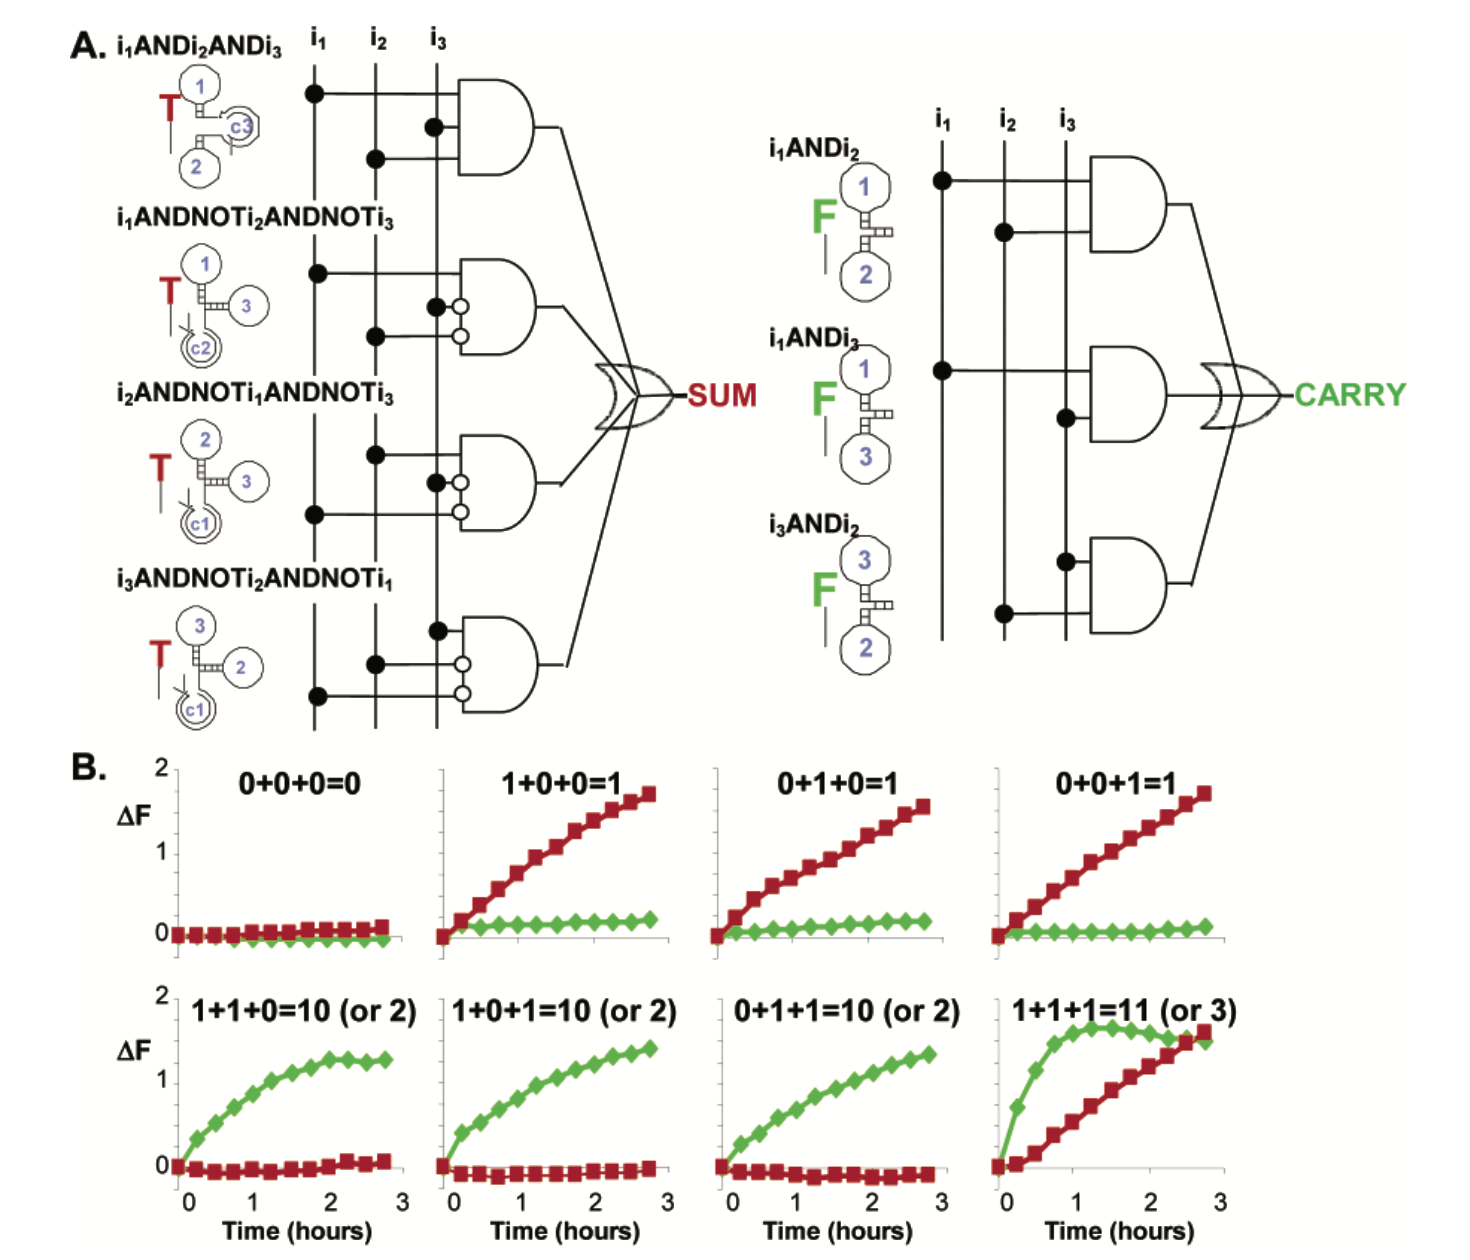
\includegraphics[width=120mm, height=120mm]{fulladder.png}
\caption{(A) Shows the deoxyribozymes required to compute the SUM and CARRY bits of the Full Adder. The proxy inputs are labelled as (c1,c2,c3) and when present they act to invert the usual response to input oligonucleotides of the corresponding stem loop. If any of the gates on the left-hand side return true the SUM bit is one. If any of the gates on the right-hand side return true the carry bit is one. (B) Shows the amount of  fluorescence (output values) for various input values (i1,i2,i3). The output for the SUM and the Carry bit fluoresce in red and green respectively \cite{Lederman2006}.}
\label{fulladder}
\end{figure}

A deoxyribozyme based molecular automaton called "MAYA" has been created. MAYA is capable of playing a perfect game of tic tac toe interactively against a human opponent. The second version of MAYA incorporates 128 deoxyribozyme logic gates. The human opponent selects a move by introducing the corresponding oligonucleotide to the system, MAYA then computes the correct response. Responses are detected using fluorescence \cite{MAYA2}.
\\
\\
DNA computation can be used in vivo for smart therapeutics (targeted drug delivery etc.) \cite{Qian11}. A development that demonstrates this is the use of a deoxyribozyme logic gate to control the opening of an aptamer (oligonucleotide that binds a specific target molecule) the deoxyribozyme computes a response based on the inputs present. If the expression is true then the deoxyribozyme cleaves the substrate holding the aptamer in its bound state. This causes the bound molecule to be released \cite{Aptamer}.

\clearpage
\subsection{Strand Displacement}
A method taking a completely different approach towards computation using DNA has been demonstrated. It uses DNA strand displacement rather than deoxyribozymes to facilitate computation \cite{enzymefree}. The logic gates created using this method are composed entirely of DNA and use oligonucleotides as both inputs and outputs. Because the outputs and inputs are both oligonucleotides the output from one computation can be used as the input for another. In this way any Boolean expression can be evaluated. As in the deoxyribozyme case high concentrations of an output molecule correspond to a true result and results are measured using fluorescence \cite{enzymefree}.

\begin{figure}[ht!]
\centering
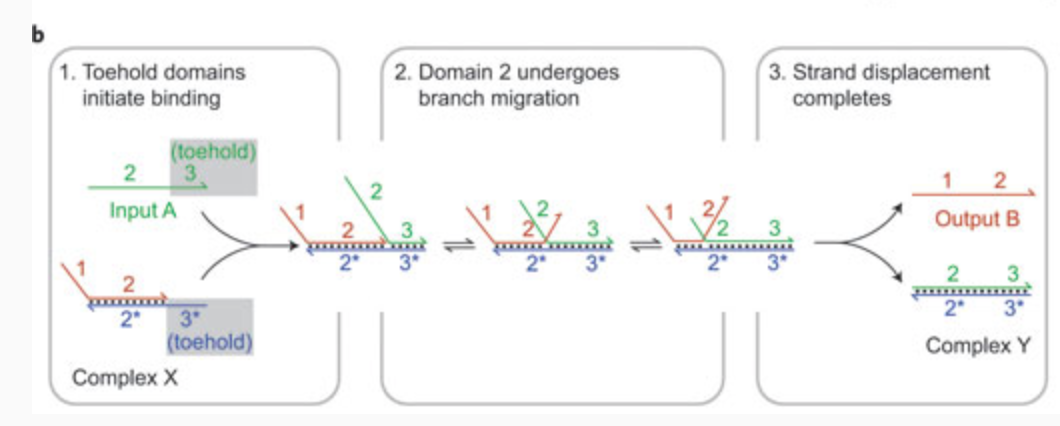
\includegraphics[width=100mm, height=60mm]{stranddisplacement.png}
\caption{Illustrates the concept of strand displacement. The complex X has an exposed single stranded region referred to as a toehold. The input A has a complementary base sequence to the toehold and also to some proportion of the rest of the complex. A binds to X at the site of the toehold, branch migration then occurs which is the process whereby A sequentially replaces the original (no toehold) strand "through a series of reversible single nucleotide dissociation and hybridization steps". Through this process an output strand B and a new complex Y containing A are created \cite{stranddisplacement}. (Y would correspond to the double stranded waste products in figure ~\ref{enzymefree}.) The rate of strand displacement can be controlled by the length and sequence of the toehold region \cite{stranddisplacement}. \label{stranddisplacement}}
\end{figure}

\clearpage
\begin{figure}[ht!]
\centering
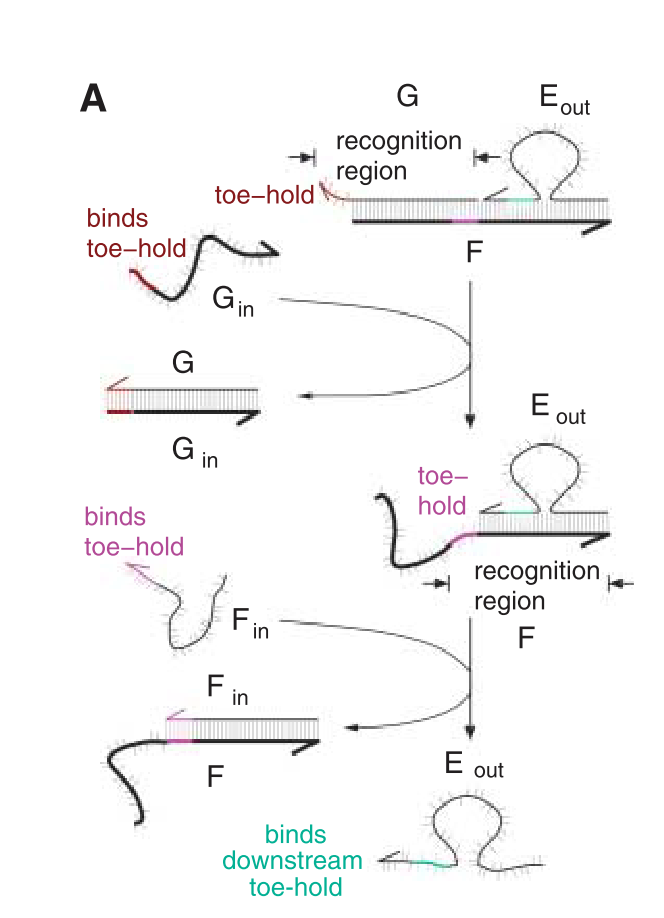
\includegraphics[width=70mm, height=90mm]{enzymefree.png}
\caption{Illustrates the process of computation for an AND gate. The AND gate is composed of an output strand Eout (only released in the presence of both input molecules), and two gate strands G,F which each contain a recognition region for the appropriate input oligonucleotide. In principle the gate can be made from any number of gate strands allowing the creation of an N-input gate. The gate is constructed such that there is an exposed toehold at the end. Gin which has a base sequence complementary to the gate strand G, can then bind with this toehold. G is then removed from the gate complex by strand displacement. This process creates a double stranded waste product (G+Gin) and exposes a toehold that Fin can bind to. Fin binds to this toehold, strand displacement occurs and the output molecule Eout is released. Eout may be an input strand that binds to the toehold of another gate or could be the final output (labelled with a fluorescent molecule) \cite{enzymefree}. OR gate functionality could be created using two single input gates each containing the same output oligonucleotide but different gate strands (different inputs). In this way, an output molecule will be released if either of the two inputs are present. \label{enzymefree}}
\end{figure}

A "circuit" that can compute the integer part of the square root of a four bit integer ($\lfloor{\sqrt{N_b}}\rfloor$) using strand displacement has been demonstrated. Gates called "seesaws" (because they are reversible) were created. Two of these seesaws (an integrating followed by an amplifying gate) can be cascaded to produce the effect of a logical OR/AND function. An integrating gate is composed of a toehold like recognition region for each input molecule. Once either input molecule is bound the output is released. In this way, a collection of integrating gates will compute the sum of the number of input molecules. An amplifying gate is composed of a toehold recognition region for the above output molecule, if this molecule binds the final output molecule is released and another toehold region is exposed. This output molecule can rebind at the newly exposed toehold creating a "seesaw" like effect (with a fuel molecule catalysing this reverse process). Amplifying gates also contain threshold molecules which contain slightly longer toe hold regions meaning they bind more quickly with the integrating gate's output molecules \cite{Qian11}. When these two bind only inert molecules with no toeholds are produced. In this way seesawing is limited until all the threshold has been bound. By using 0.6 $\times$ standard concentration (in this case 100nMol) threshold molecules the final output molecules will be produced if either input molecule is present (OR gate), however if the amount of threshold used is instead 1.2 $\times$ standard concentration then the final output molecules will only be produced if both inputs are present. Again output molecule presence is detected using fluorescence. By chaining these logic operations together, the circuit in question was created \cite{Qian11}.

\clearpage
\subsection{Algorithmic Self-Assembly}
The final method that will be discussed is computation through the self-assembly of DNA tiles. It has been demonstrated that these tiles can be used to compute a cumulative XOR operation on a 4 bit string \cite{Tiles00}. A DNA triple crossover tile is illustrated in figure ~\ref{dnatiles}(a) it consists of 4 single strands of DNA bound together such that 3 helical domains develop. The arrows indicate locations of sticky ends (unpaired bases that anneal to complementary strands) which are the locations at which the tile structure grows. In figure ~\ref{dnatiles}(b) we see the tiles that are used in this computation. The green C1 and C2 tiles are the initialisation tiles at which the initial input tiles bind. The 2 blue tiles (X) act as inputs (0, 1). The red tiles (Y) act as the outputs of the XOR operation, there are 4 tiles because there are 2 ways to reach each answer for an XOR gate so the binding sites on the ends of the tiles need to reflect this. Because of the structure of the tiles the first X tile used will cause a Y tile of the same value to bind ($X_1=Y_1$). Any further binding will follow $Y_i=Y_{i-1}$ XOR $X_i$ with each subsequent introduction of an input X tile. Figures ~\ref{dnatiles}(c) and ~\ref{dnatiles}(d) are examples of the tile structure that can develop (the number on each tile indicates its Boolean value). Figure ~\ref{dnatiles}(e) shows how the tile structure develops in strand form. The red strand that runs through the entirety of this structure is called the reporter strand and it encodes the value of all the inputs and outputs. To access this information the reporter strand is replicated using PCR (only primers for the possible endings of the reporter strand are used). Two restriction endonucleases (cleaves the phosphodiester bonds in a double strand to create two double strands\cite{paun2013DNA}) that act at two different recognition regions (one region corresponding to logical 1 and the other to logical 0) are introduced separately. The two solutions are then run through gel electrophoresis, to determine the outputs and inputs.\cite{Tiles00}.
\begin{figure}[ht!]
\centering
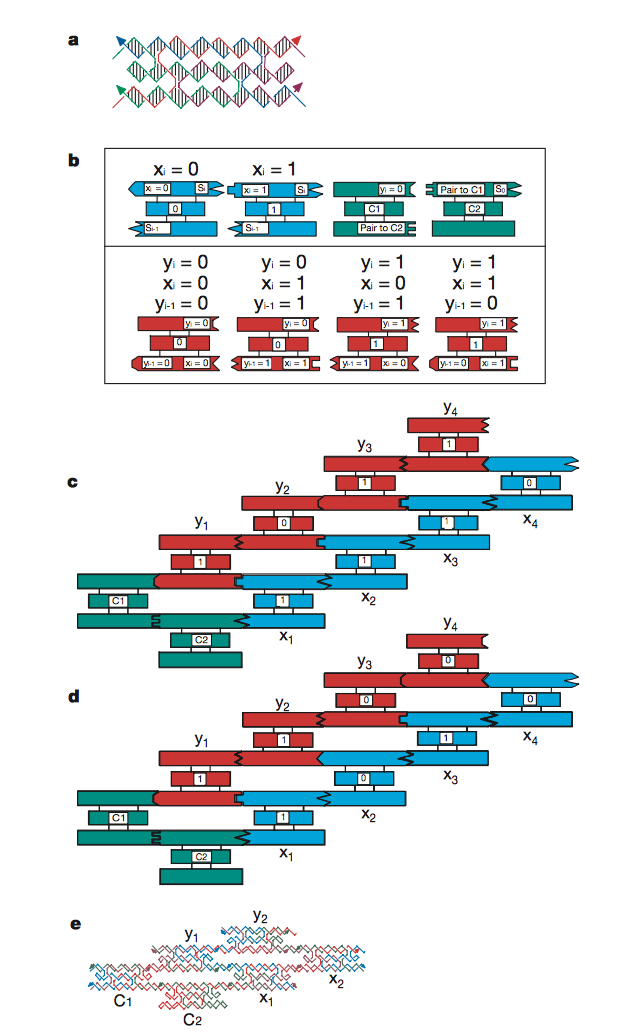
\includegraphics[width=80mm, height=120mm]{dnatiles.png}
\caption{Illustrates triple crossover tiles and the structures they can create. \cite{Tiles00}  \label{dnatiles}}
\end{figure}
\\
\\
A possible application of this technique is the "algorithmically directed self-assembly of intricate patterns and smart materials" \cite{Tiles00} If the above method could be extended to create 2D/3D patterns of output Y tiles then in principle it would be possible to create nanoscale patterns/materials algorithmically rather than through more direct manipulation methods \cite{Tiles00}. A method similar to the one outlined above has been used to generate Sierpinkski's triangle (a 2D pattern) algorithmically \cite{Sierpinski}.

\clearpage
\section{Advantages and Limitations}
\subsection{Advantages}
\begin{itemize}
\item DNA computation can be carried out in vivo \cite{Qian11}.
\item Very energy efficient \cite{Adleman1994}\cite{Ezziane06}.
\item Extremely high memory density ~$10^{20}$ Bytes $cm^{-3}$ \cite{Adleman1994}\cite{Ezziane06}.
\item Massive parallelisation capabilities \cite{Adleman1994}\cite{Ezziane06}.
\end{itemize}

\subsection{Disadvantages}
\begin{itemize}
\item Error rates higher when copying information in comparison to traditional computers \cite{Ezziane06}.
\item Harder to analyse the results of computations (often needs human intervention), must use labelling techniques fluorescence etc. \cite{Adleman1994}\cite{DeoxyribozymeLogic}\cite{enzymefree}\cite{Tiles00}.
\item Computation speeds of Boolean operations can be quite slow \cite{Lederman2006}\cite{MAYA2}.
\item The strands that are used have to be tailor made for their purpose. Resources are finite and need to be replenished to repeat calculations \cite{Adleman1994}.
\end{itemize}

\clearpage
\section{Other Applications}
\title{Storing information using DNA}
DNA can also be used as an incredibly dense information storage medium \cite{DNAstorage}. A benefit of using DNA to store information is that it has properties which make it extremely suitable for long term storage \cite{Cox2001}.  A possible application of DNA storage is in an associative/content addressable memory. \cite{Baum583} In a standard storage solution such as in a conventional hard drive you need to know the physical address of a piece of information before you can retrieve it. In associative storage you can retrieve information through partial knowledge of its content (fix a complementary strand to a magnetic bead, strands containing this information will bond and can therefore be retrieved\cite{Baum583}). Deletion, creation and copying are easily implemented through obvious operations on the solution. Preserving DNA for extensive lengths of time (millions of years) could be accomplished by encasing it inside a spore and then storing the spores in Amber or an artificial resin. \cite{Cox2001} 


\clearpage
\section{Conclusions}
All of these computational methods are effective information processing techniques. The principle benefit of processing information using DNA is its potential to carry out computation in vivo \cite{Ezziane06}. It appears as though each of the methods have a particular function that they would be best suited for. Deoxyribozymes have the potential to interact with other downstream components (aptamers) through their cleavage action \cite{Aptamer}, so seem to be the most suitable form of computation for targeted drug delivery systems as they can interact directly with the drug binding molecule. The strand displacement method when used to create "seesaw" like logic gates has the benefit that the gate components are reusable and can be powered by a replenishable fuel \cite{Qian11}, strand displacement also has an added benefit in that it can take RNA as an input so can be adapted for in situ detection of RNA \cite{enzymefree}. The "seesaw" method may be the most suitable for general computation as the components are reusable. And finally, the tiles method seems to be useful for producing complex structures, as it directly produces patterns algorithmically through its computation method \cite{Tiles00}. Each of these methods have their own strengths and weaknesses and future applications will most likely use a combination of these methods. The particular method employed will depend on the desired function of the application. 
\clearpage
\printbibliography
\end{document}